% Preamble
\documentclass[xcolor=dvipsnames]{beamer}
\usetheme{madrid}

% Packages
\usepackage[english,ngerman]{babel}
\usepackage[utf8]{inputenc}
\usepackage{amsmath}
\usepackage{graphicx}
\usepackage{ifthen} % Boolean variables

\definecolor{hBlue}{RGB}{55,118,165}
\usecolortheme[named=hBlue]{structure}

% Distiction between work and stream presentation
\newboolean{work}
\setboolean{work}{true}

\ifthenelse{\boolean{work}}{
    \titlegraphic{
\includegraphics[width=4cm]{../images/logo.png}}
}{}
\title{Gesundheit \& Ernährung}
\subtitle{Fette}
\ifthenelse{\boolean{work}}{
    \author{Adrian Helberg}
    \date{09.06.2021}
}{
    \subtitle{twitch.tv/bl1nzlar}
    \author{Bl1nzlar}
    \date{\today}
}


% Document
\begin{document}

    \maketitle

    \frame{\frametitle{Agenda}\tableofcontents}

    \section{Theorie}
    {
    \setbeamercolor{normal text}{fg=hBlue}\usebeamercolor*{normal text}
    \begin{frame}
        \begin{center}
            \Huge Theorie
        \end{center}
    \end{frame}
    }

    \subsection{Profil und Fakten}
    \begin{frame}[allowframebreaks]
        \frametitle{Fettprofil und fette Fakten}
        \begin{block}{Profil}
            \begin{itemize}
                \setlength\itemsep{1em}
                \item kleinste Bausteine: Fettsäuren
                \item Unterscheidung in Anzahl Kohlenstoffatome und Doppelbindungen
                \item 10-12 häufige Fettsäuren, 400 weitere Strukturen
                \item Vorkommen als Triglyceride in der Pflanzenwelt
                \item Fettsäuren werden in Form von Triglyzeriden im Fettgewebe gespeichert
                \item Triglyzeride werden mit der Lipolyse wieder in Fettsäuren zerlegt
            \end{itemize}
        \end{block}

        \framebreak

        \begin{figure}
            \centering
            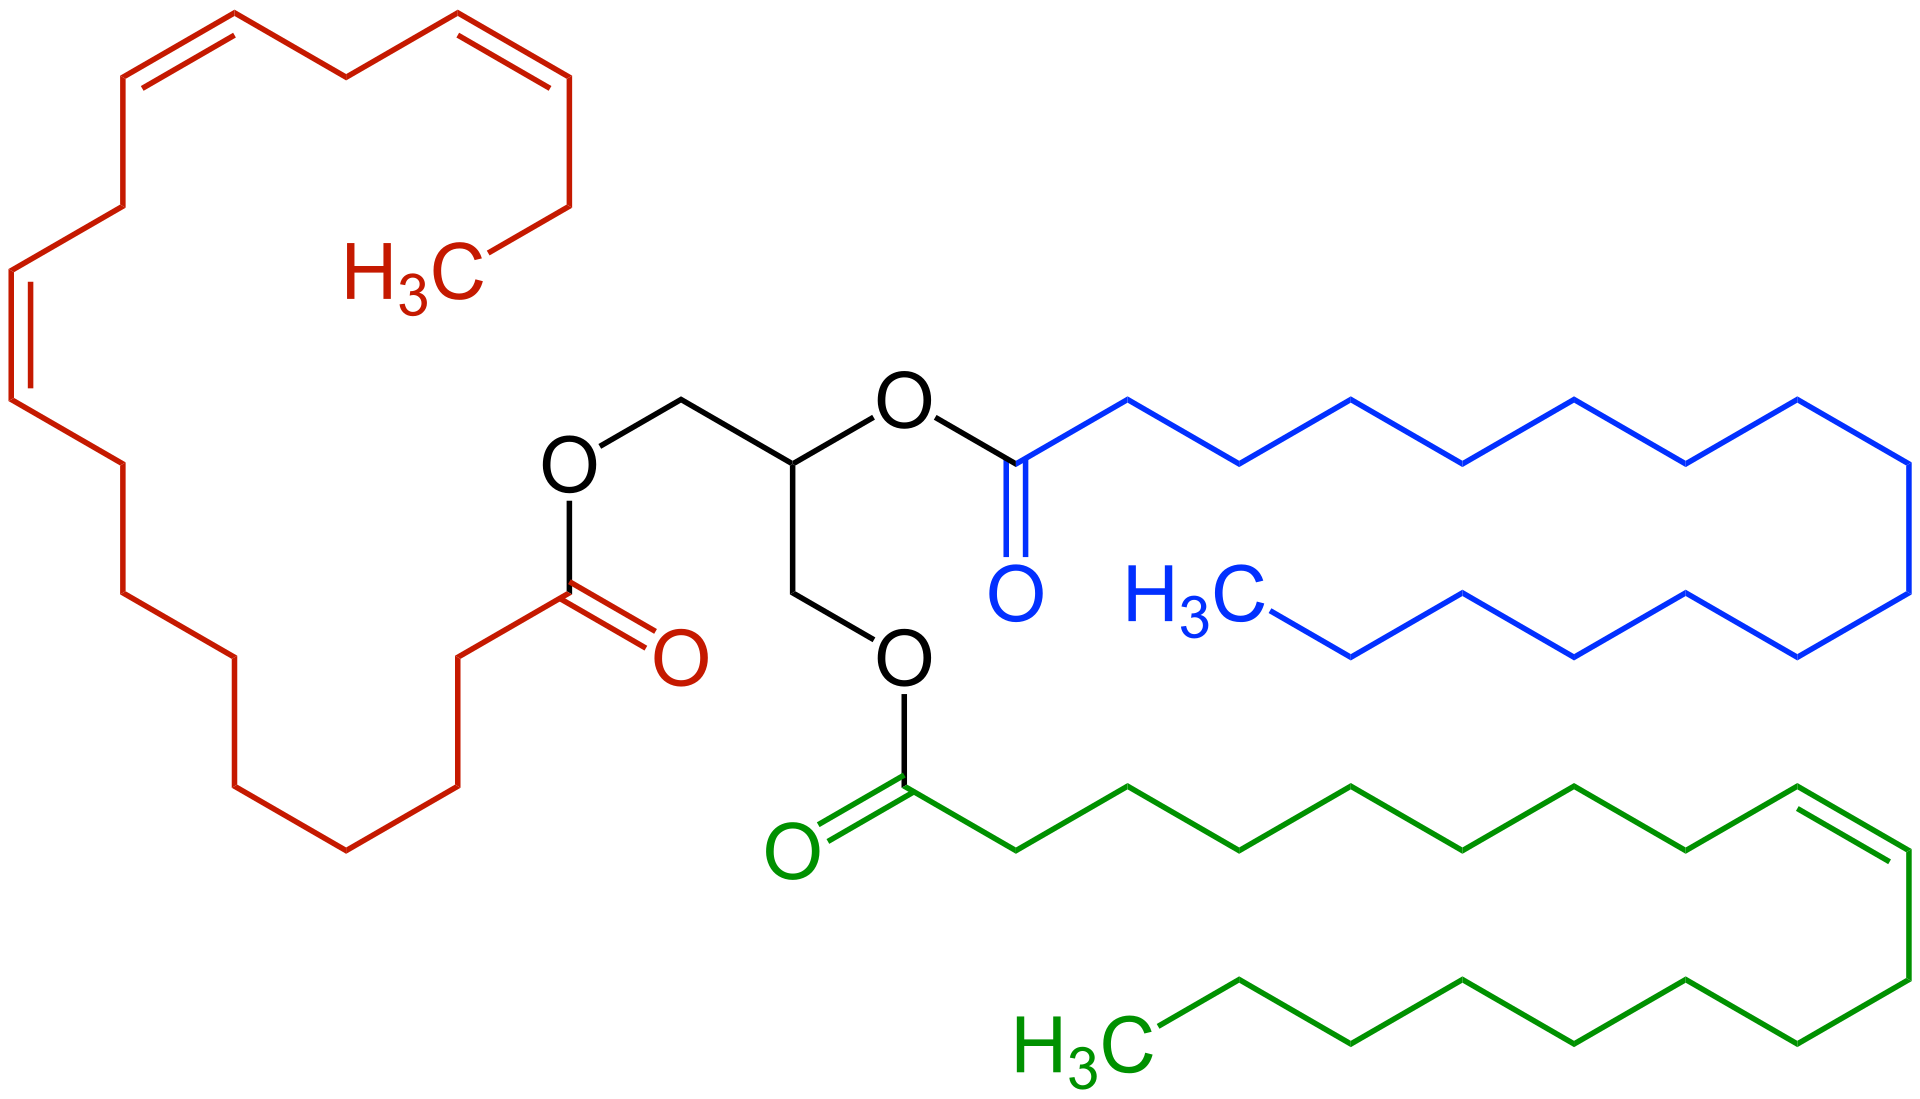
\includegraphics[width=10cm]{../images/Triglyzerid.png}
            \caption{Triglyzerid (blau: gesättigt, grün: einfach ungesättigt, rot: mehrfach ungesättigt)}
        \end{figure}

        \framebreak

        \begin{block}{Fakten}
            \begin{itemize}
                \setlength\itemsep{1em}
                \item Fett macht nicht fett
                \begin{itemize}
                    \setlength\itemsep{1em}
                    \item Nahrungsfett $\neq$ Körperfett
                    \item Hormonstörungen und Entzündungen machen dick und krank
                \end{itemize}
                \item Dosis und Qualität von Fettsäuren ist wichtig
                \begin{itemize}
                    \setlength\itemsep{1em}
                    \item "`Vorsichtige"' Herstellung
                    \item BIO-Siegel
                    \item Kaltpressung
                    \item Ausschluss von Licht, Hitze und Sauerstoff (Oxidation)
                \end{itemize}
                \item Fett macht schlau, schlank und gesund
            \end{itemize}
        \end{block}
    \end{frame}

    \subsection{Qualitätsmerkmale}
    \begin{frame}
        \frametitle{Qualitäten von Fett}
        \begin{block}{Die richtige Dosis und Qualität von Fetten führt zu\ldots}
            \begin{itemize}
                \setlength\itemsep{1em}
                \item exzelenter Energieversorgung
                \item vielfältigen Geschmäckern (Geschmacksträger)
                \item guter Vitaminversorgung
                \item langem, erfüllendem Sättigungsgefühl
            \end{itemize}
        \end{block}
    \end{frame}

    \subsection{Nahrungsfette}
    \begin{frame}[allowframebreaks]
        \frametitle{Nahrungsfette - Mindmap}
        \begin{figure}{}
            \centering
            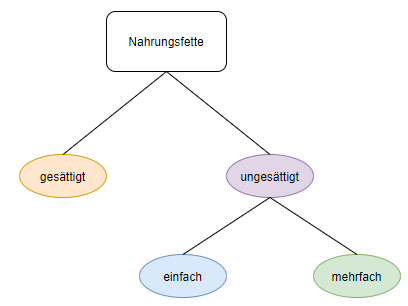
\includegraphics[width=5cm]{../images/Fette_Kategorisierung.png}
            \caption{t}
        \end{figure}

        \framebreak

        \begin{figure}{}
            \centering
            \includegraphics[width=8cm]{../images/Fette_Kategorisierung_gesättigt.png}
            \caption{t}
        \end{figure}

        \framebreak

        \begin{figure}{}
            \centering
            \includegraphics[width=8cm]{../images/Fette_Kategorisierung_ungesättigt.png}
            \caption{t}
        \end{figure}

        \framebreak

        \begin{figure}{}
            \centering
            \includegraphics[width=8cm]{../images/Fette_Kategorisierung_ungesättigt_einfach_mehrfach.png}
            \caption{t}
        \end{figure}
    \end{frame}

    \subsection{Fettsäureprofile}
    \begin{frame}
        \frametitle{Fettsäureprofile}

        \begin{figure}{}
            \centering
            \includegraphics[width=10cm]{../images/Fettsäurenprofil_2.png}
            \caption{Fettsäureprofil einiger Fette}
        \end{figure}
    \end{frame}

    \subsection{N-kettige Fettsäuren}
    \begin{frame}[allowframebreaks]
        \frametitle{N-kettige Fettsäuren}

        \begin{block}{Kurzkettige Fettsäuren (SCFA = Short Chain Fatty Acids)\ldots}
            \begin{itemize}
                \setlength\itemsep{1em}
                \item werden von Bakterien im Darm gebildet unter Zufuhr von Ballaststoffen
                \begin{itemize}
                    \item Obst, Gemüse, Hülsenfrüchte, Kartoffeln, etc.
                \end{itemize}
                \item regulieren das Körpergewicht
                \item vermindern das Darmkrebsrisiko
                \item erhöhen Insulinempfindlichkeit
                \item sind entzündungshemmend
            \end{itemize}
        \end{block}

        \framebreak

        \begin{block}{Mittelkettige Fettsäuren (MCFA = Middle Chain Fatty Acids)\ldots}
            \begin{itemize}
                \setlength\itemsep{1em}
                \item MCTs (medium chain triglycerides) sind gesättigt
                \begin{itemize}
                    \item Butter, Kokosfett, Palmfett, etc.
                \end{itemize}
                \item wird bei Darmerkrankungen genutzt
            \end{itemize}
        \end{block}

        \framebreak

        \begin{block}{Langkettige Fettsäuren (LCFA = Long Chain Fatty Acids)\ldots}
            \begin{itemize}
                \setlength\itemsep{1em}
                \item
                \begin{itemize}
                    \item Ölsäure, Olivenöl
                \end{itemize}
            \end{itemize}
        \end{block}

    \end{frame}

    \section{Praxis}
    {
        \setbeamercolor{normal text}{fg=hBlue}\usebeamercolor*{normal text}
        \begin{frame}
            \begin{center}
                \Huge Praxis
            \end{center}
        \end{frame}
    }

    \subsection{Test}
    \begin{frame}
        \frametitle{Test}
    \end{frame}

    \section{Fragerunde}
    {
        \setbeamercolor{normal text}{fg=hBlue}\usebeamercolor*{normal text}
        \begin{frame}
            \begin{center}
                \Huge Fragerunde
            \end{center}
        \end{frame}
    }

\end{document}
